\documentclass[11pt,handout]{beamer}
\usetheme{Goettingen}
\usecolortheme{dolphin}
%\usetheme{Goettingen}

\AtBeginSection[]{
  \begin{frame}
  \vfill
  \centering
  \begin{beamercolorbox}[sep=8pt,center,shadow=true,rounded=true]{title}
    \usebeamerfont{title}\insertsectionhead\par%
  \end{beamercolorbox}
  \vfill
  \end{frame}
}

\usepackage[utf8]{inputenc}
\usepackage[english]{babel}
\usepackage{amsmath}
\usepackage{amsfonts}
\usepackage{amssymb}
\usepackage{graphicx}
\usepackage{xcolor}
\author{Lino AA Notarantonio}
\title{Fundamentos de Econometr\'ia \\ Introducción}
%\setbeamercovered{transparent} 
%\setbeamertemplate{navigation symbols}{} 
%\logo{} 
%\institute{} 
%\date{} 
%\subject{} 
\begin{document}


\begin{frame}
\titlepage
\end{frame}

%\begin{frame}[allowframebreaks] \tableofcontents \end{frame}

%\begin{frame}{\'Indice}\pause 

%\begin{enumerate}[<+->]
%	\item Modelos econ\'omicos v. modelos econométricos
%	\item Modelos econom\'etricos
%	\item Estructura de los datos econ\'omicos
%	\item Causalidad (''Ceteris Paribus'')
%	\item Modelos de regresi\'on lineal
%	\begin{enumerate}
%		\item Simple
%		\item M\'ultiple
%	\end{enumerate}
%\end{enumerate}
%\end{frame}

\section{Metodología de trabajo}


\begin{frame}{Organización del trabajo a lo largo de la UF}
{Política de las actividades}

\begin{itemize}
	\item En cada sesión,  se podrán asignar grupos de trabajo de forma aleatoria. 

	\item Se entiende por trabajo cualquier actividad que pueda contribuir a la calificación final. 

	\item La asignación de trabajos podrá ocurrir en cualquier momento de la sesión de 2 horas. 
	
	\item No se aceptarán trabajos tardíos.
	
	\item No hay reposición de trabajos.  
\end{itemize}

\end{frame}

\section{Modelo Económico v. modelo econométrico}

\begin{frame}{Modelación}

Un economista laboral quiere estudiar qu\'e factores son importantes en la productividad de ciertos trabajadores.

\vspace{.5cm}
Algunos factores que pueden impactar la productividad son

\begin{itemize}[<+->]
	\item educaci\'on, $educ$;
	\item experiencia, $exper$; 
	\item capacitaci\'on; $capac$.
\end{itemize}

\end{frame}

\begin{frame}{Modelo econ\'omico vs  modelo econométrico}

El \alert{modelo económico} es una función
\[
	wage = f(educ, exper, capac)
\]
y  se analizan las consecuencias de la forma matemática de la función: entre otros
\begin{itemize}
	\item relaciones directa/inversa entre las variables dependiente e independientes;
	
	\item elasticidades;
	
	\item retornos constantes a escala
\end{itemize}

\vspace{.25cm}
El \alert{modelo econométrico} \textbf{estima}, numérica y estadísticamente, la relación entre las variables.

\end{frame}

\begin{frame}{Modelo econ\'omico vs  modelo econométrico}

\pause 
\textbf{Modelo económico} Existe una relación directa entre el número de hora de capacitación y el salario de los trabajadores de cierta industria.

\pause  \vspace{.25cm}
\textbf{Modelo econométrico} Un aumento en un 20\% en el número de horas de capacitación para los trabajadores de cierta industria aumentará el salario de estos trabajadores en \$1,500 por quincena. 

 \end{frame}

\begin{frame}{Econometría} 

\textbf{Definición de Econometría} (Samuelson \textit{et al.}, 1954)
\begin{quotation}
	[A]pplication of mathematical statistics to economic data to lend 
empirical support to models constructed by mathematical economics 
and to obtain numerical estimates.
\end{quotation}

\pause \vspace{.125cm}
\textbf{Problemas} 
\pause 
\begin{itemize}[<+->]
	\item Obtener conclusiones correctas a partir de un muestra, en lugar de la población entera:
		\begin{itemize}[<+->]
			\item muestreo aleatorio;
			\item inferencia estadística.
		\end{itemize}
	\item Resumen estadístico, de manera que los resultados cuantitativos se puedan interpretar de manera comprensible y concisa.
\end{itemize}
\end{frame}

\begin{frame}{Modelo econométrico}
{Formulación}

En un modelo econométrico se deben considerar otros posibles factores que puedan afectar la variable dependiente que no se consideran explicitamente en el modelo
%Otros factores pueden afectar el salario 
$\Rightarrow$ \textcolor{red}{término de error}:
\pause 
\[
	wage = \beta_0 + \beta_1 educ + \beta_2 exper + \beta_3 capac + \textcolor{red}{u}
\]
\end{frame}

\begin{frame}{Modelo econométrico}
{Formulación}

\[
	\textcolor{olive}{wage} = \beta_0 + \beta_1 \textcolor{blue}{educ} + \beta_2 \textcolor{blue}{exper} + \beta_3 \textcolor{blue}{capac} + \textcolor{red}{u}
\]
\begin{itemize}
	\item \textcolor{blue}{variables explicativas} del modelo.
	\item \textcolor{olive}{variable explicada}.
	\item \textcolor{red}{error} ó \textcolor{red}{variables no observables}.
	\item $\beta_1$,  $\beta_2$, $\beta_3$: pendientes
	\item $\beta_0$: intercepto
%	\begin{itemize}
%		\item El t\'ermino de error se conoce también como factores diferentes a los mencionados, que pero pueden tener un efecto importante en la variable explicada (habilidades de uno; familia; etc.)
%	\end{itemize}
\end{itemize}


\end{frame}

\begin{frame}
{Modelo econométrico}{Terminología}

\begin{center}

\begin{tabular}{|c|c|}
\hline 
$y$ & $x$ \\ 
\hline 
variable depediente & variable independiente \\ 
\hline 
variable explicada & variable explicativa \\ 
\hline 
variable de respuesta & variable de control  \\ 
\hline 
variable predicha & variable predictora \\ 
\hline 
regresando & regresor \\ 
\hline 
\end{tabular} 

\end{center}

\end{frame}

\begin{frame}{Modelo econométrico}
{Comentarios}

Considera el modelo
\[
wage  = \beta_0 + \beta_1 educ  + \beta_2 exper + \beta_3 capac + u
\]

\begin{itemize}[<+->]
	\item Si estamos interesados en el efecto del entrenamiento sobre el salario, entonces el par\'ametro de inter\'es es $\beta_3$
	\item Si pensamos que la experiencia no afecta el salario de una persona, entonces se debe verificar que $\beta_2=0$
	\item Si postulamos que la educaci\'on tiene un efecto positivo sobre el salario, entonces se debe mostrar que $\beta_1>0$
\end{itemize}

\vspace{.25cm}
¿Cómo se puede interpretar $\beta_0$?
\end{frame}

\section{Estructura de los datos económicos}

\begin{frame}{Estructura de los datos econ\'omicos}
\pause
\begin{itemize}[<+->]
	\item Datos de corte transversales
	\item Series de tiempo
	\item Combinaciones de cortes transversales
	\item Datos tipo panel (longitudinales)
\end{itemize}
\end{frame}


\begin{frame}
{Datos de corte transversal}
\pause 
Se obtienen mediante un muestreo aleatorio de la poblaci\'on de inter\'es, en alg\'un momento en el tiempo.
\end{frame}

\begin{frame}
{Series de tiempo}
\pause 
\begin{itemize}[<+->]
	\item Observaci\'on de una o m\'as variables a lo largo de un periodo de tiempo
	\item Es importante el ordenamiento temporal de los datos
	\item La frecuencia de observaci\'on tambi\'en es importante (p.ej., factores estacionales)
\end{itemize}
\end{frame}

\begin{frame}
{Combinaci\'on de cortes transversales}
\pause 
Se lleva a cabo una encuenta de cortes transversales de las familias de cierta ciudad. \pause Pasado cierto periodo de tiempo, la misma encuesta considera otra muestra de las familias.
\pause
\begin{itemize}[<+->]
	\item Para incrementar el tama\~no de la muestra, se combinan las dos encuestas (\textit{Pooled Cross Sections})
	\item Una combinaci\'on de cortes transversal es muy \'util para verificar el efecto de una pol\'itica, por ejemplo (antes y despu\'es)
\end{itemize}
\end{frame}

\begin{frame}
{Datos tipo panel}
\pause 
Datos tipo panel son series de tiempo para cada corte transversal de la base de datos. 
\end{frame}

\section{Causalidad (Ceteris Paribus)}

\begin{frame}
{Causalidad}

Preguntas típicas: 
\pause 
\begin{itemize}[<+->]
	\item Si el banco central aumenta la tasa de interés, ¿qué pasará con el costo de las hipotecas? 
	\item Si tomo este curso de capacitación, ¿en cuánto aumentará mi salario?
	\item Si el gobierno federal invierte en la costrucción de autopistas, ¿en cuánto aumentará el PIB?
	\item Si aumentara el costo de una cajetilla de cigarros, ¿cuánto será el porcentaje de disminución de los fumadores?
\end{itemize}
\pause 
En todas estas preguntas es claro cuál es la causa y cuál es el efecto. 

% \pause \vspace{.125cm} La teoría económica permite justificar una relación de causalidad. 
\end{frame}

\begin{frame}
{Ceteris Paribus y experimentos}

\pause 
\begin{quote}
	Si los precios aumentan, entonces los consumidores comprarán menos, \alert{manteniendo constantes los demás factores.} 
\end{quote}
\pause 

\begin{itemize}
	\item Si los demás factores no se mantienen constante, entonces todo puede pasar. 

	\item Un experimento puede verificar la existencia de un vínculo causal entre un factor y otro. 

	\item En los últimos 30 años la Economía se ha enriquecido mediante el uso de modelo experimentales; en el 2019 Abhijit Banerjee, Esther Duflo, and Michael Kremer ganaron el Premio Nobel\footnote{Más precisamente, The Sveriges Riksbank Prize in Economic Sciences in Memory of Alfred Nobel.}
	\href{https://www.nobelprize.org/prizes/economic-sciences/2019/press-release/}{\textcolor{blue}{“for their experimental approach to alleviating global poverty"}}.
	% el campo de \emph{Behavioural Economics} ha permitido desarrollar Economía se pueden diseñar experimentos 
	%Ciencias Sociales puede ser muy difícil diseñar y llevar a cabo experimentos controlados para establecer un vínculo causal. 
\end{itemize}
\end{frame}

%\begin{frame} {Causalidad y Econometría}

%\begin{itemize}[<+->]
%	\item En las disciplinas experimentales se pueden establecer vínculos causales mediante experimentos controlados.
%	\item En econometría se manejan, por lo general, datos observados (no experimentales). 
%	\item Las herramientas econométricas \textbf{no} se usan para establecer vínculos causales; éstos se justifican en la teoría económica. La econometría permite \textbf{cuantificar} los vínculos causales y/o verificar su presencia. 
%\end{itemize}
%\end{frame}

\begin{frame}{Ceteris Paribus: Modelación}
{Wooldridge, Ejemplo 2.1}

\pause 
Considera el modelo
\[
	rendimiento = \beta_0 + \beta_1 fertilizante + u
\]
\pause 
A un investigador agr\'icola le puede interesar conocer el efecto del fertilizante sobre el rendimiento de las parcelas. 

¿Cómo puede el investigador justificar el análisis \emph{ceteris paribus}?

\pause \vspace{.25cm}
%Si las cantidades de fertilizante se eligen independientemente de otras caracter\'isticas de las parcelas, entonces es posible justificar el análisis \textit{ceteris paribus}.
%la ecuaci\'on 
%\[	E[u|x] = E[u] (=0) \]
%es v\'alida.
\end{frame}

\begin{frame}{Correlación y causalidad}

\textcolor{blue}{\href{http://tylervigen.com/}{Correlación no implica causalidad}}

\end{frame}

\begin{frame}{Ejemplo}

\begin{columns}[T] % align columns
\begin{column}{.48\textwidth}
% \color{red}\rule{\linewidth}{4pt}
% Left Part

\textbf{Variables}: $ingreso$ (disponible), $gasto$ (del hogar)

\begin{center}
	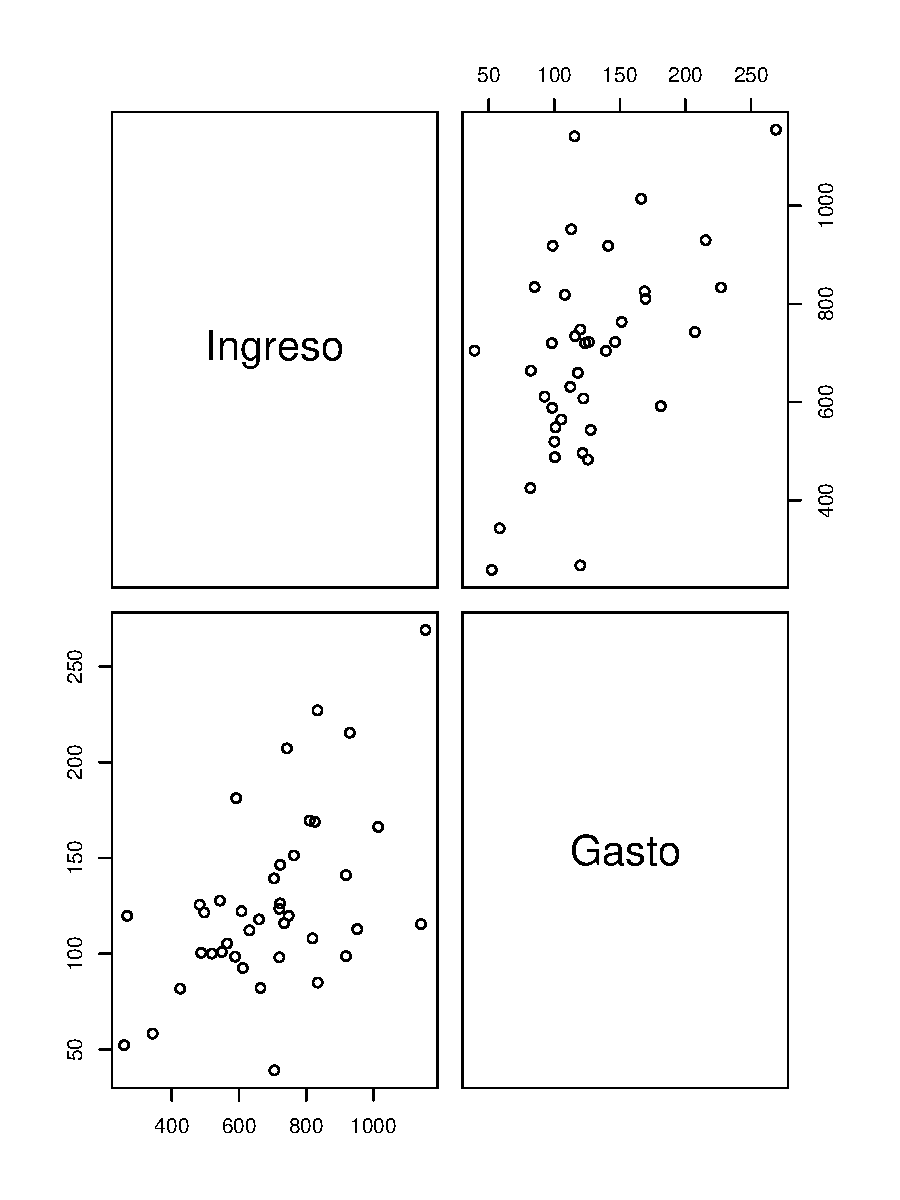
\includegraphics[scale=.3]{fig1.pdf} 
\end{center}


\end{column}%
\hfill%
\begin{column}{.48\textwidth}
%\color{blue}\rule{\linewidth}{4pt}
%Right Part

\begin{itemize}

	\item ¿Qué signo de la \alert{correlación}, $corr(ingreso, gasto)$, esperamos? 

	\item ¿Qué tipo de relación esperamos entre estas variables (directa; inversa)?

	\item ¿Cuál es la variable \alert{dependiente}?

\end{itemize}

\end{column}%
\end{columns}

\end{frame}

\begin{frame}
{Diferencia entre correlación y regresión}

\pause 

\begin{itemize}[<+->]
	\item La \textbf{correlación} mide el grado de dependencia lineal entre dos variables.
	\item La regresión (lineal) \textbf{cuantifica} una relación \textbf{causal} entre la variable dependiente y las variables independientes.
	\item Un modelo de regresión \alert{no} establece una relación causal entre la variable dependiente y la(s) variable(s) independiente(s).  
%	\item Un modelo econométrico no se puede usar para establecer una relación causal entre variables (regresiones espurias). 
	\item Una relación causal se puede establecer mediante experimentos controlados.  	
\end{itemize}

\end{frame}

\section{Métodos de Mínimos Cuadrados Ordinarios}


\begin{frame}
{Modelo de regresión simple}

Un modelo (econométrico) que relacione $inc$, $gasto$ es
\[
	gasto = \textcolor{blue}{\beta_0} + \textcolor{blue}{\beta_1} inc \alert{+ u}. %, \quad i=1,\ldots, n
\]
%(Modelo de regresión simple)

\begin{itemize}[<+->]
%	\item $n$ es el \textbf{tamaño muestral} de los valores observados de ingreso, gasto.
	\item $u$: modela la presencia del ruido en la medición de las variables.
	% es el \textbf{error}, que modela factores no observados que pueden también influir en $gasto$. 
	\item  En el modelo, los parámetros $\textcolor{blue}{\beta_0}$, $\textcolor{blue}{\beta_1}$ son incógnitos.
	\item La \alert{estimación} de $\textcolor{blue}{\beta_0}$, $\textcolor{blue}{\beta_1}$ se realiza usando 
	\alert{muestras aleatorias} de las variables en el modelo.
	\item Los parámetros estimados se indican con $\textcolor{blue}{\widehat{\beta}_0}$, $\textcolor{blue}{\widehat{\beta}_1}$ y son \textcolor{blue}{variables aleatorias}. 
	\item Modelo estimado (ó recta de regresión estimada)
		\[
			\boxed{
				\alert{\widehat{gasto} = \widehat{\beta}_0 + \widehat{\beta}_1 inc}
			}
		\] 
%		La \alert{recta de regresión estimada} (modelo estimado)
%	\item Por lo tanto, la variable $gasto$ es \alert{aleatoria}.
%	\item El modelo econométrico arriba se conoce como \textbf{modelo de regresión simple}. 

\end{itemize}

\end{frame}

\begin{frame}
{Modelo econométrico}{Terminología}

En el modelo 
\[
	y = \beta_0 + \beta_1 x + u
\]
el término 
\pause 
\begin{itemize}[<+->]
	\item $\beta_0$ se conoce como el \textbf{intercepto};
	\item $\beta_1$ como la \textbf{pendiente}.
	\item Bajo ciertas condiciones, 
		\[ 
			\beta_1 = \frac{\Delta y}{\Delta x}, 
		\]
		es la \alert{función marginal} (derivada) de $y$ con respecto a $x$. 
	\item Función marginal: $\Delta y$, cuando $\Delta x = 1$.
\end{itemize}

\end{frame}

\section{Estimación por mínimos cuadrados ordinarios (MCO)}

\begin{frame}
{Justificación}

\pause 

%\textbf{Problema} 
Usar muestra aleatoria $(x_i, y_i)$ para estimar $\beta_0$, $\beta_1$:

\pause 
\vspace{-2cm}
\begin{center}
	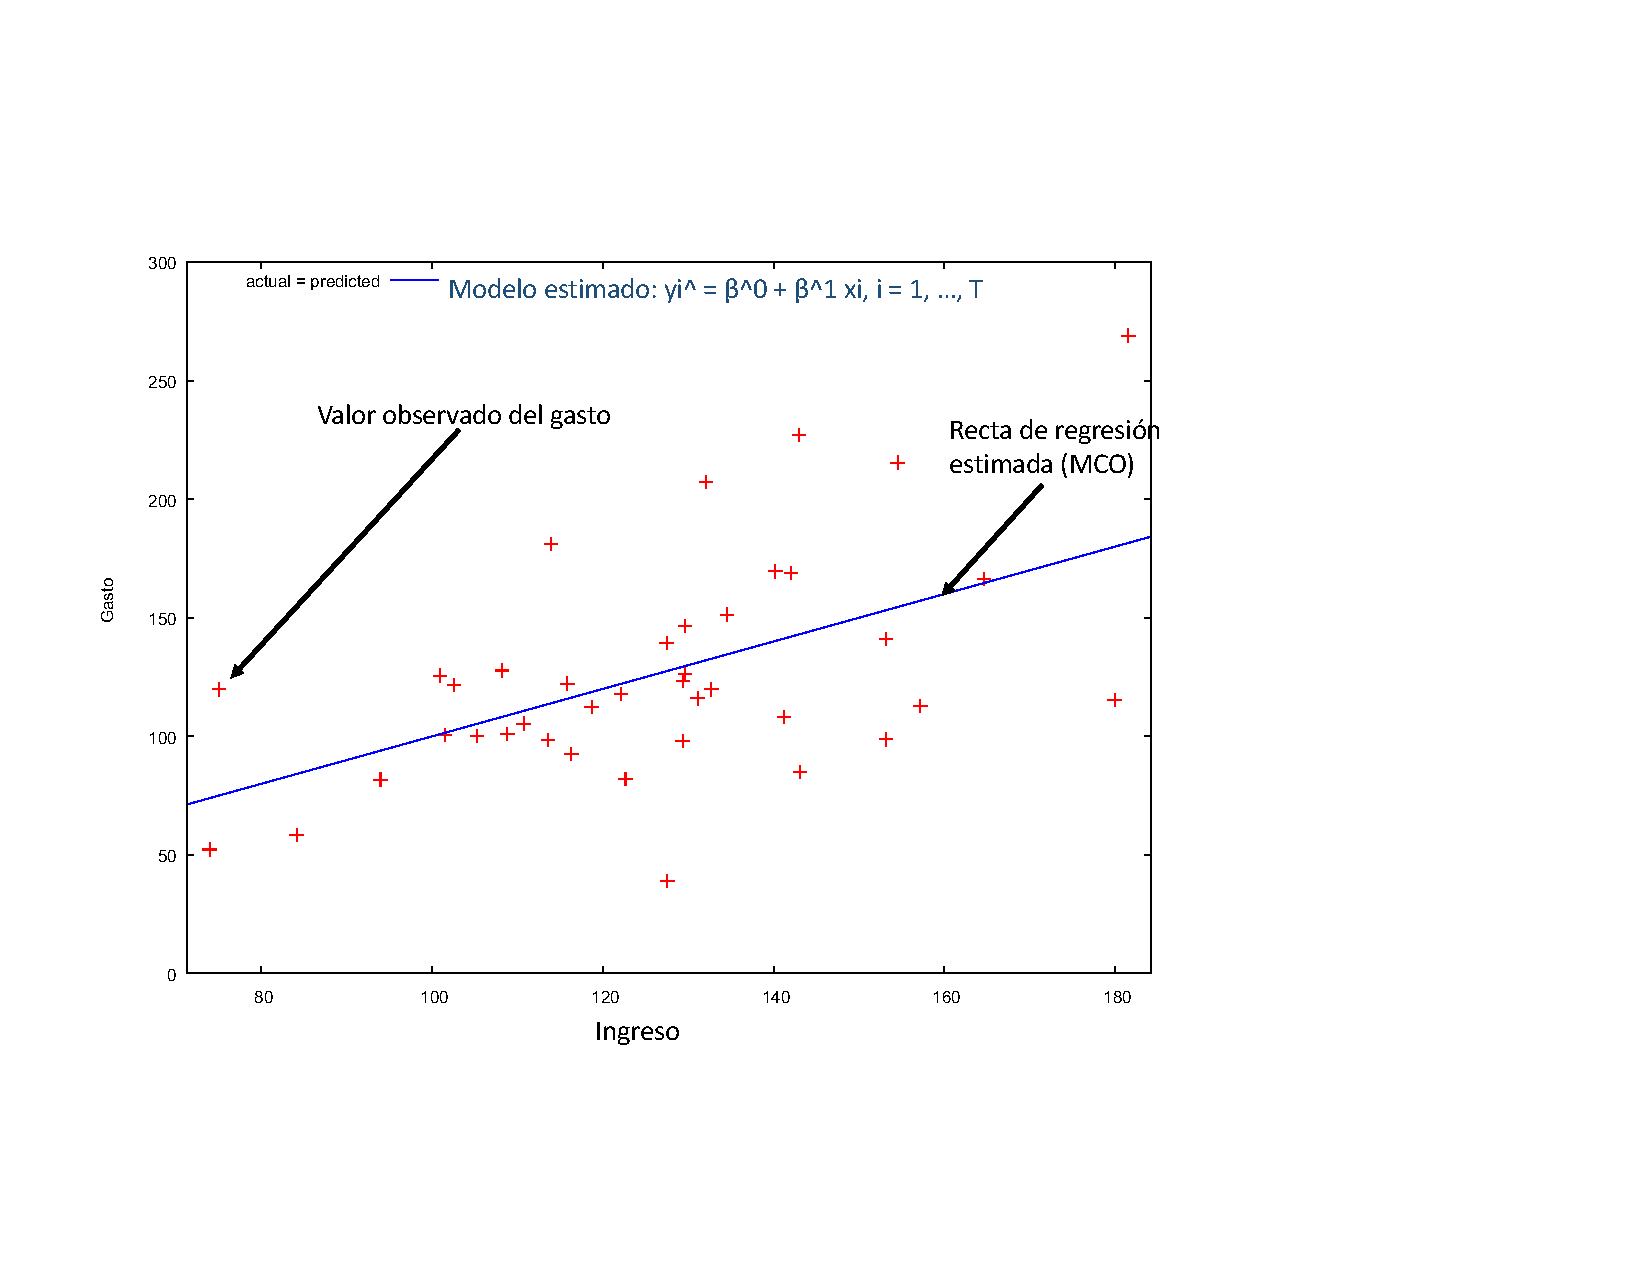
\includegraphics[scale=.45]{fig2-1.pdf} 
\end{center}

\end{frame}

\begin{frame}
{Justificación}

\pause 

%\textbf{Problema} 
Usar muestra aleatoria $(x_i, y_i)$ para estimar $\beta_0$, $\beta_1$:

\pause 
\vspace{-2cm}
\begin{center}
	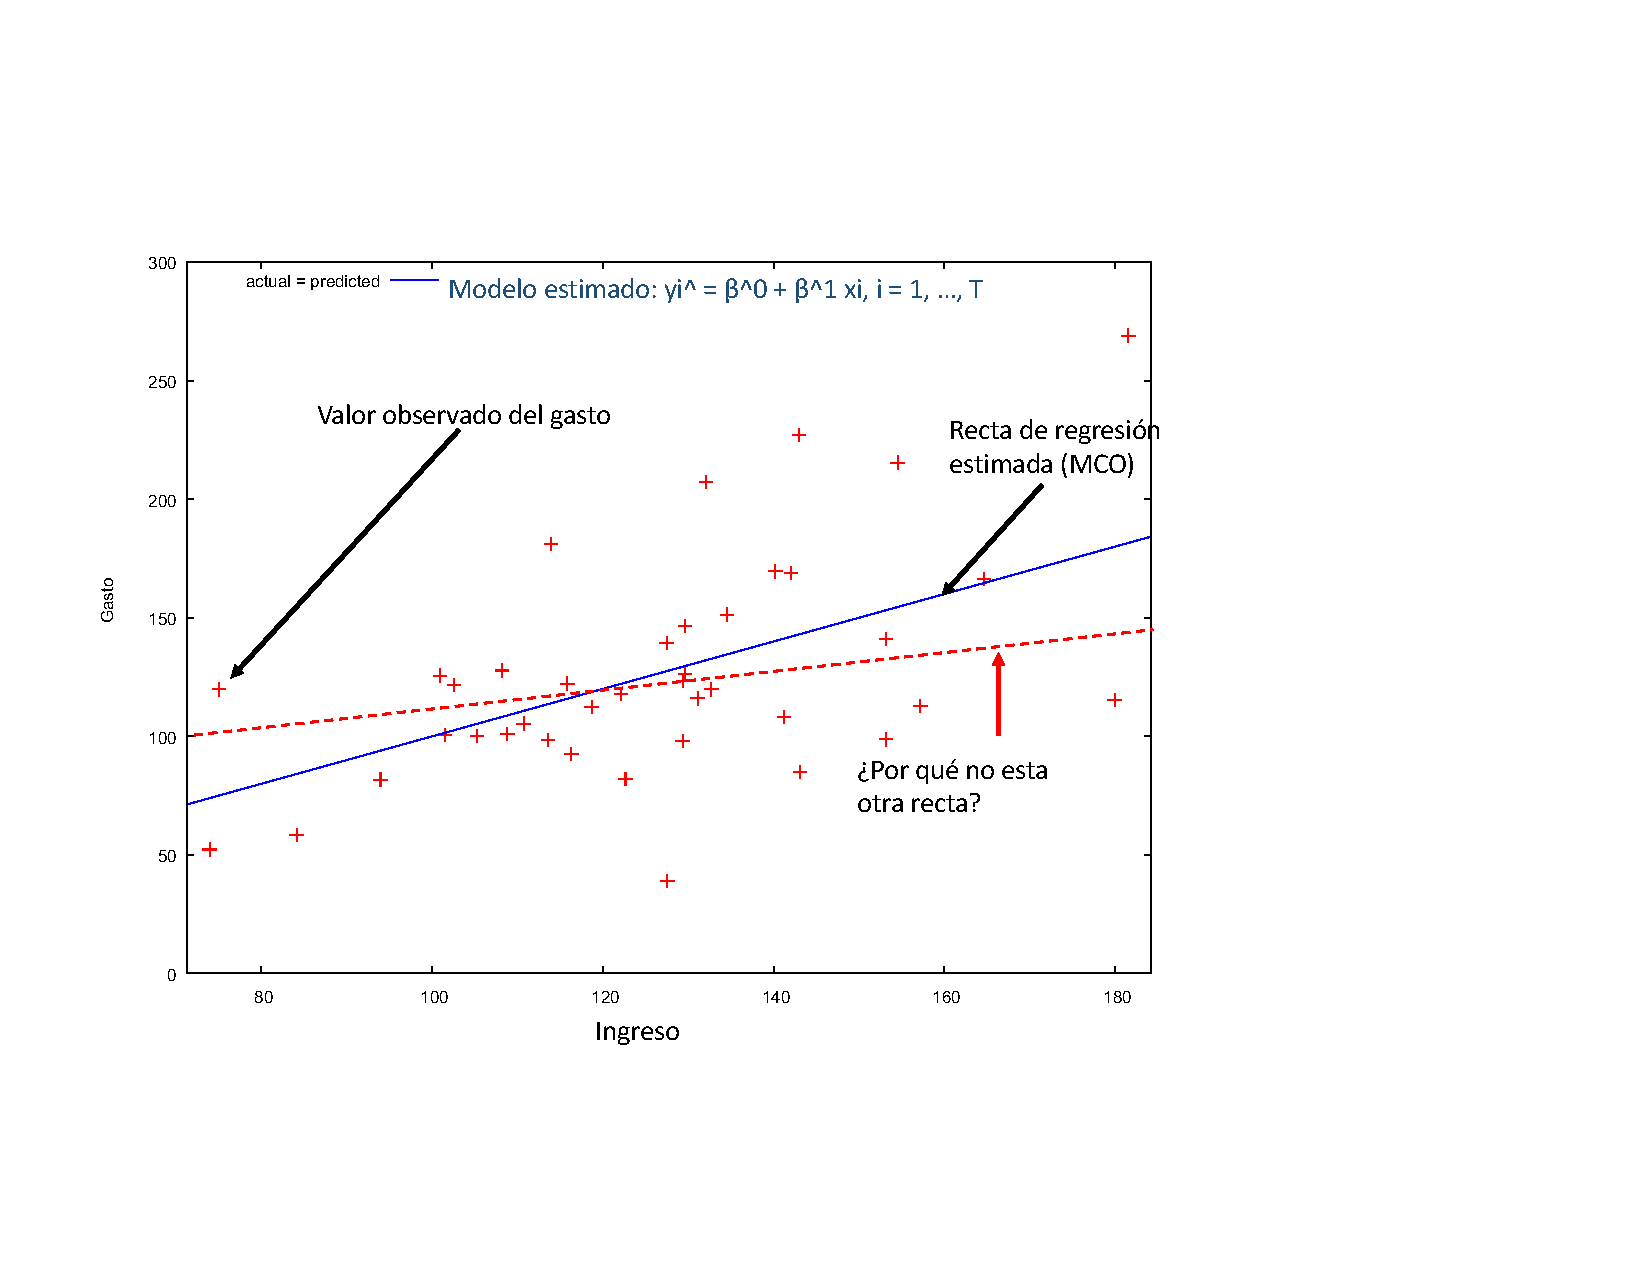
\includegraphics[scale=.45]{fig2-11.pdf} 
\end{center}

\end{frame}

\begin{frame}
{Justificación}

\pause 

%\textbf{Problema} 
Usar muestra aleatoria $(x_i, y_i)$ para estimar $\beta_0$, $\beta_1$:

\pause 
\vspace{-2cm}
\begin{center}
	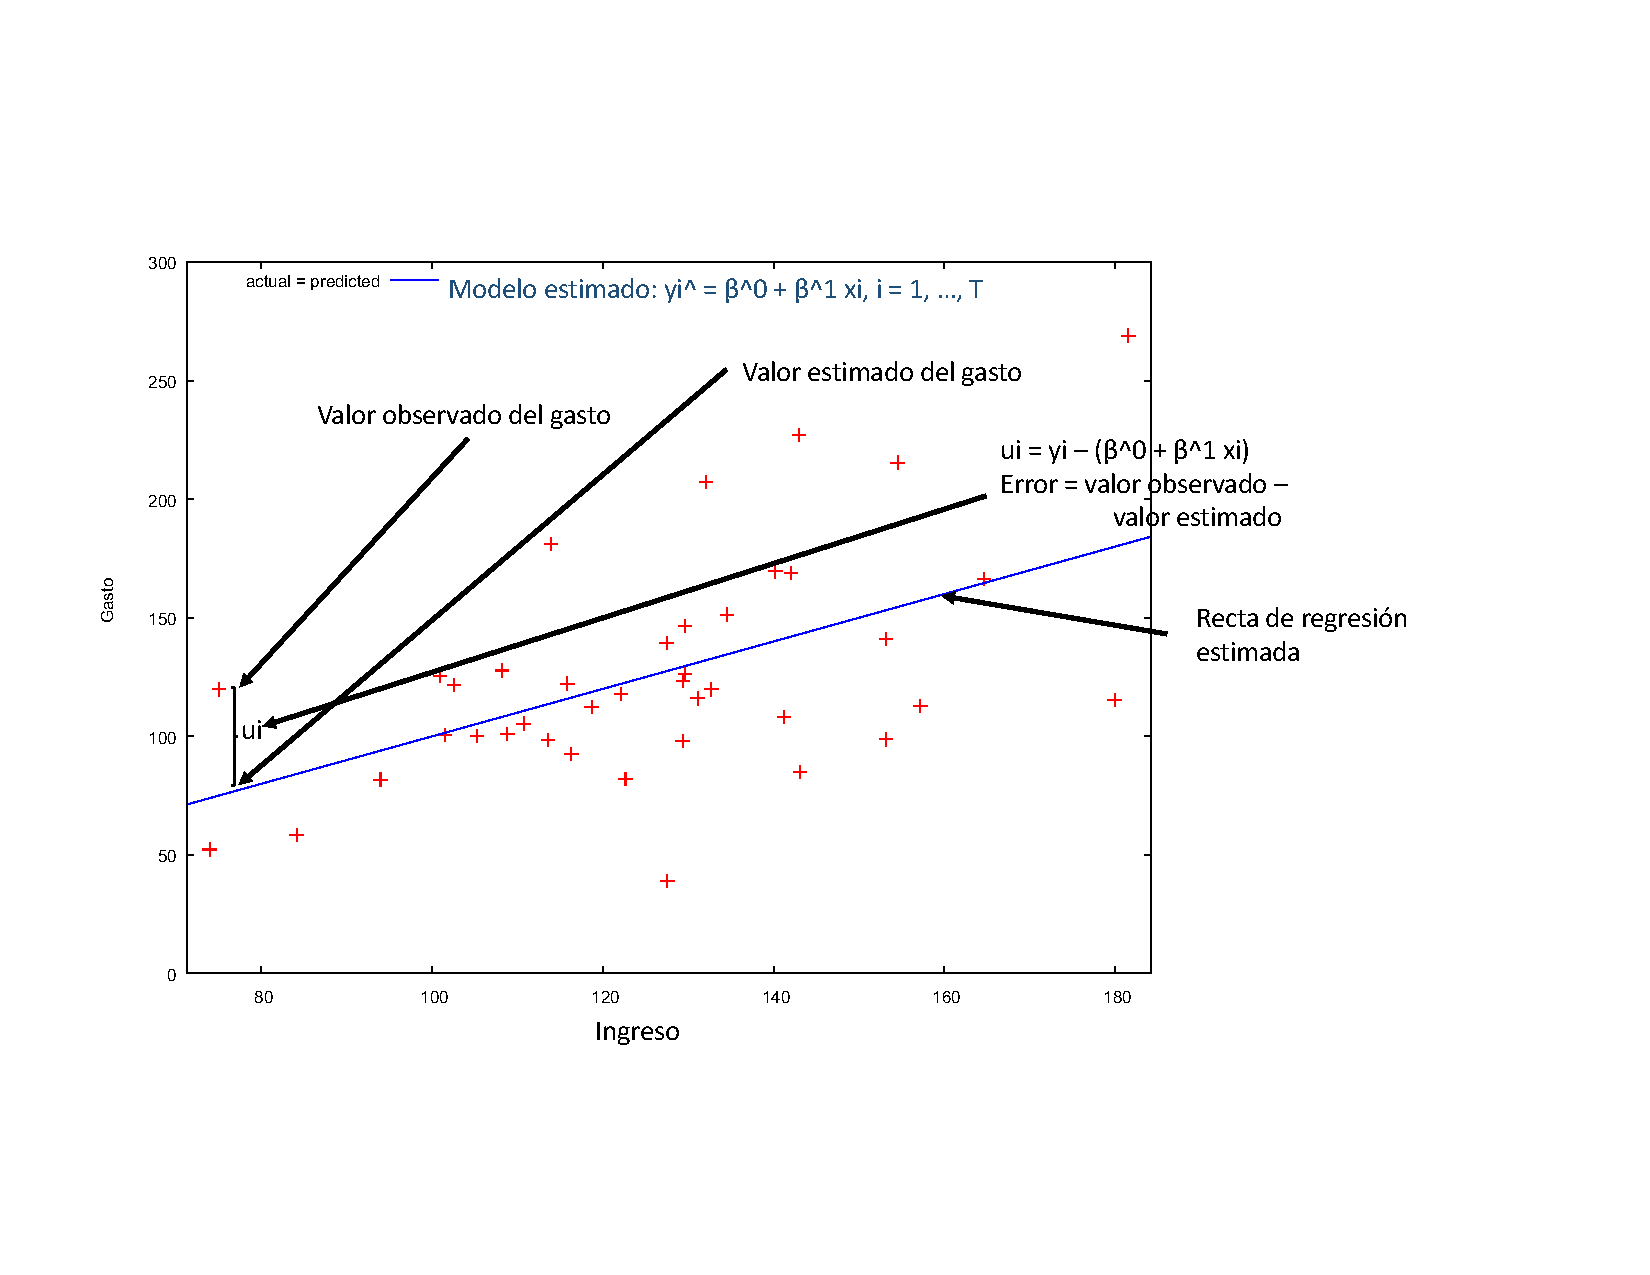
\includegraphics[scale=.45]{fig2-2.pdf} 
\end{center}

\end{frame}

\begin{frame}
{Justificación}

\pause 

%\textbf{Problema} 
Usar muestra aleatoria $(x_i, y_i)$ para estimar $\beta_0$, $\beta_1$:

\pause 
\vspace{-2cm}
\begin{center}
	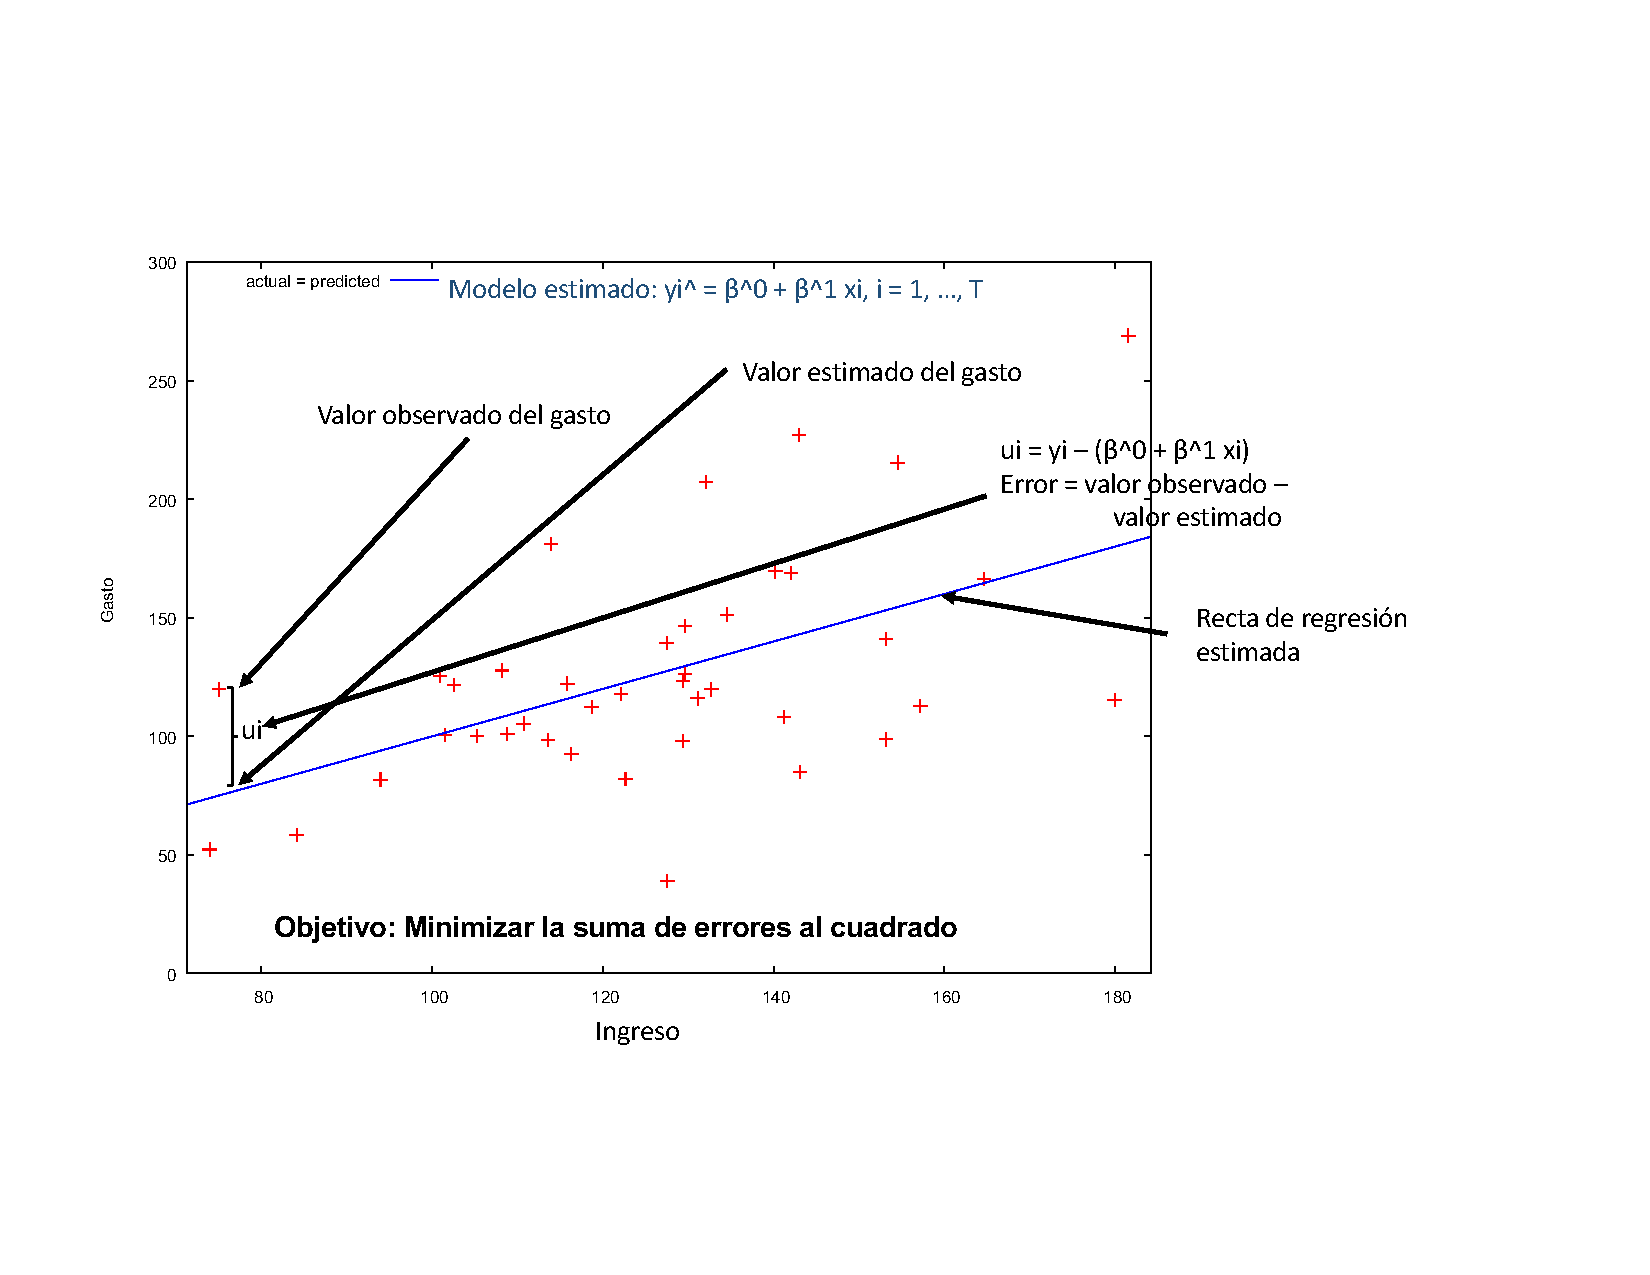
\includegraphics[scale=.45]{fig2-3.pdf} 
\end{center}

\end{frame}

\begin{frame}
{Fórmula de los estimadores}

%\pause 
%Error: $u_i = y_i - (\beta_0 + \beta_1 x_i)$
%\pause \vspace{.5cm}
Usando una muestra aleatoria $(x_i, y_i)_{i=1}^n$ de tamaño $n$, se minimiza la suma de los cuadrados de los errores:
\[
	\min\sum_{i=1}^n u_i^2 = \boxed{
		\min_{\textcolor{blue}{\beta_0}, \textcolor{blue}{\beta_1}} \left\lbrace
		\sum_{i=1}^n \left[ y_i - (\textcolor{blue}{\beta_0} 
			+ \textcolor{blue}{\beta_1} x_i)  \right]^2
			\right\rbrace}
\]
Función de $\textcolor{blue}{\beta_0}$, $\textcolor{blue}{\beta_1}$:
\[
	f(\textcolor{blue}{\beta_0}, \textcolor{blue}{\beta_1}) = 
	\sum_{i=1}^n \left[ y_i - (\textcolor{blue}{\beta_0} 
	+ \textcolor{blue}{\beta_0} x_i)  \right]^2
\] 
La función se minimiza usando cálculo (puntos críticos; concavidad de la función)

\end{frame}

\begin{frame}
{Fórmula de los estimadores}


El mínimo de la función se logra en los valores:
\begin{align*}
	\widehat{\beta}_0 & = \overline{y} - \widehat{\beta}_1 \overline{x} \\
	& \\
	\widehat{\beta}_1 & = \frac{\sum_{i=1}^n (x_i-\overline{x}) (y_i-\overline{y}) }{\sum_{i=1}^n (x_i-\overline{x})^2} ,
\end{align*}
($\overline{x}$, $\overline{y}$ son las medias muestrales de $x$, $y$, respectivamente.)  

\begin{itemize}
	\item El valor de los estimadores $\widehat{\beta_0}$, $\widehat{\beta_1}$ depende de la muestra $(x_i, y_i)$: los estimadores son variables aleatorias.
	
	\item El valor de los estimadores depende de manera lineal de $y$.
\end{itemize}

\end{frame}



\begin{frame}
{Medición de ajuste}

\begin{itemize}
	\item $\displaystyle{ SRC = \sum (\widehat{u}_i)^2}$ \qquad \alert{Suma Residuos Cuadrados}
	\item $\displaystyle{ STC = \sum (y_i - \overline{y})^2}$ \qquad \alert{Suma Total de Cuadrados}
	\item $\displaystyle{ SEC = \sum (\widehat{y}_i - \overline{y})^2}$ \qquad \alert{Suma Explicada al Cuadrado}
	\item Siempre se cumple
		\[
			STC = SEC + SRC
		\]
\end{itemize}

\end{frame}

\begin{frame}
{Medición de ajuste}

\begin{align*}
	STC = SEC + SRC &\Rightarrow SEC = STC - SRC \\
			& \Rightarrow \frac{SEC}{STC} = 1 - \frac{SRC}{STC}
\end{align*}

\begin{align*}
	R^2 &  = \frac{SEC}{STC} \\
			& = 1 - \frac{SRC}{STC} 
\end{align*}

\begin{itemize}
	\item $R^2$ mide el porcentaje de variación de $y$ explicado por $x$. 
	
	\item Equivalentemente,  $R^2$ mide el porcentaje de ajuste del modelo.

	\item El valor de $R^2$ siempre se da como decimal.
\end{itemize}

\end{frame}

\section{Actividad 1}

\begin{frame}{Actividad 1}{Wooldridge, Problema 1, p. 17}
	Suponga que se le pide que realice un estudio para determinar si grupos de clase pequeños contribuyen a un mejor desempeño de los estudiantes de cuarto grado. 
	
	\begin{itemize}
		\item Si pudiera reallizar cualquier experimento que deseara, ¿qué haría? Explique con claridad.
		
		\item Siendo más realista, suponga que puede obtener datos observacionales de varios miles de estudiantes de cuarto grado de un determinado estado. Puede conocer el tamaño de sus grupos y las calificaciones estandardizadas obtenidas en el examen final. \\ ¿Por qué puede esperarse una correlación negativa entre el tamaño de los grupos y las puntuaciones en el examen final?
\end{itemize}

\end{frame}

\begin{frame}{Actividad 1}{Wooldridge, Problema 1, p. 17}

\begin{itemize}		
		\item Una correlación negativa, ¿indicaría necesariamente que tamaños de grupos menores causan un mejor desempeño? Explique.
\end{itemize}

\vspace{.25cm}

\textbf{Entrega} Miércoles, 24 de marzo, 09:00AM en un documento Word, que se subirá a Canvas.  

La solución se subirá a Canvas, el mismo miércoles, a las 11:00 horas. 
\end{frame}

\end{document}

\section{Modelos de regresión lineal simple}

%\subsection{Terminología}

\begin{frame}{Modelo de regresi\'on simple}
\pause 
Sean $x$, $y$ dos variables. 
\pause
Se quiere explicar $y$ en t\'ermino de $x$:
\[
	y = \beta_0 + \beta_1 x + u
\]
\pause
Esta relaci\'on se conoce como modelo de \textbf{regresi\'on lineal simple}. 
\end{frame}

\begin{frame}{Terminolog\'ia}
\pause 
\centerline{
\begin{tabular}{|c|c|}
\hline 
$y$ & $x$ \\ 
\hline 
variable dependiente & variable independiente \\ 
\hline 
variable explicada & variable explicativa \\ 
\hline 
variable de respuesta & variable de control \\ 
\hline 
variable predicha & variable predictora \\ 
\hline 
regresando & regresor \\ 
\hline 
\end{tabular} 
}
\end{frame}

\begin{frame}{Modelo de regresi\'on simple}
\pause 
\[
	y = \beta_0 + \beta_1 x + u
\]
%Si los factores no observables se mantienen constantes, $\Delta u=0$, entonces la relaci\'on entre $y$, $x$ es lineal. 
La relación entre $x$, $y$ es lineal, \textit{ceteris paribus} (\textit{i.e.}, si $\Delta u=0$)\pause,  es decir si $u$ no depende de $x$.
\pause 
\begin{itemize}[<+-| alert@+>]
	\item $\beta_0$ se conoce como (\textbf{par\'ametro de}) \textbf{intercepto} (t\'ermino constante)
	\item $\beta_1$ se conoce como (\textbf{par\'ametro de la}) \textbf{pendiente}. 
%	\item La pendiente $\beta_1$ mide el efecto de $x$ sobre $y$, cuando $\Delta u=0$. 
	\item $\Delta y = \beta_1 \Delta x$, si $\Delta u=0$. 
	\item Sin pérdida de generalidad, $E[u]=0$.
\end{itemize}
\end{frame}

\section{Supuestos de Gauss-Markov}

\begin{frame}{Supuestos de Gauss-Markov}
{Modelo Lineal Clásico}

%Los siguientes supuestos están a la base de la teoría econométrica. 
\pause 
	\begin{description}[<+->]
		\item[RL1] El modelo de regresión es \textbf{lineal} en los \textcolor{magenta}{parámetros}:
		\[
			y = \textcolor{magenta}{\beta_0} + \textcolor{magenta}{\beta_1} x + u .
		\]
		\item[RL2] Se cuenta con una muestra aleatoria de tamaño $n$, $(x_i,y_i)$, que sigue el modelo poblacional.
		\item[RL3] $Var(x)\not =0$.%, es decir, los valores observados $(x_i)$ no son todos iguales. 
		\item[RL4] $E(u|x)=0$, es decir, los factores no observados, $u$, \textbf{son media independientes} del factor observado $x$. 
		\item[\textcolor{red}{RL5}] \textcolor{red}{$Var(u|x) = \sigma^2$ %, esto es, la varianza de los factores no observados es \textbf{constante} 
				(\textbf{Homocedasticidad}).}
		\item[\textcolor{olive}{RL6}] \textcolor{olive}{Los factores no observados $u \sim N(0,\sigma^2)$.
		%Los factores no observados tienen distribución normal, con $E(u)=0$, $Var(u) = \sigma^2$.
		}
	\end{description}

\end{frame}

\begin{frame}{Comentarios sobre los supuestos de Gauss-Markov}

\pause 
	\begin{description}[<+->]
		\item[RL4] $E(u|x) = 0$ es la formulación matemática de la noción \textit{ceteris paribus}. 
		
		\item[RL4] Si $E(u|x) \not= 0$, entonces se dice que el modelo 
		\[
			y = \beta_0 + \beta_1 x + u
		\]
		presenta \textbf{correlación espuria}. La prueba RESET de Ramsey puede ayudar a eliminar correlaciones espurias. 
			
		\item[RL5] $Var(u|x) = \sigma^2$ es equivalente a $Var(y|x) = \sigma^2$. 
	\end{description}

\end{frame}


\subsection{Función de Regresión Poblacional (FRP)}

\begin{frame}{Modelo de regresi\'on simple}
\pause 
De las dos relaciones 
\begin{align*}
E[u|x] & = 0 \\ %E[u] \\
y & = \beta_0 + \beta_1 x + u 
\end{align*}
\pause se obtiene la \textbf{funci\'on de regresi\'on poblacional} (FRP)
\[
	E[y|x] = \beta_0 + \beta_1 x
\]
\end{frame}

\begin{frame}{Modelo de regresi\'on simple}

%Usando la FRP  \[	E[y|x] = \beta_0 + \beta_1 x \] se reconoce que la pendiente, $\beta_1$, corresponde al valor esperado del cambio en la variable $y$ cuando $\Delta x =1$. 
\pause 
La suposici\'on de causalidad, \alert{RLS4}, divide la ecuaci\'on de regresi\'on en dos partes:
\pause 
\begin{itemize}[<+-| alert@+>]
	\item La \textbf{parte sistem\'atica}, $E[y|x] = \beta_0 + \beta_1 x$, que es la parte de la regresi\'on explicada por $x$
	\item La \textbf{parte no sistem\'atica}, $u$, que corresponde a la parte de $y$ no explicada por $x$
\end{itemize}
\pause 
\end{frame}

\subsection{Método de Mínimos Cuadrados Ordinarios (MCO)}

\begin{frame}{M\'etodo de M\'inimos Cuadrados (MCO)}

Se usarán los supuestos RLS1 a RLS4 para \alert{estimar} los parámetros del modelo de regresión
\[
	y = \textcolor{red}{\beta_0} + \textcolor{red}{\beta_1} x + u
\]
\end{frame}

\begin{frame}{M\'etodo de M\'inimos Cuadrados (MCO)}

\pause 
%Considera el modelo de regresi\'on simple
%\[ 	y = \beta_0 +\beta_1 x + u \]
Usando RLS 4 ($E[u]=0$),
%\pause 
\[
\text{Cov}(u,x)=0\quad\Rightarrow\quad  E[xu]=0
\]
por lo que 
\pause 
\begin{enumerate}[<+-| alert@+>]
	\item $E[u] = E[y-\beta_0-\beta_1 x] = 0$
	\item $E[xu] = E[x(y-\beta_0-\beta_1 x)] = 0$
\end{enumerate}
\pause 
\end{frame}

\begin{frame}{M\'etodo de M\'inimos Cuadrados (MCO)}

\pause Mediante muestreo aleatorio (RLS2) el método de momentos permite escribir %determinar estimadores $\widehat{\beta_0}$, $\widehat{\beta_1}$ de $\beta_0$, $\beta_1$, respectivamente,
%, respectivamente, que resuelvan las contropartes muestrales de las ecuaciones dadas arriba:
\pause 
\begin{enumerate}[<+-| alert@+>]
	\item $\displaystyle{\frac{1}{n}\sum_{i=1}^n \left(y_i- \textcolor{red}{\widehat{\beta_0}} - \textcolor{red}{\widehat{\beta_1}} x_i\right) = 0}$
	\item $\displaystyle{\frac{1}{n}\sum_{i=1}^n x_i\left(y_i - \textcolor{red}{\widehat{\beta_0}} - \textcolor{red}{\widehat{\beta_1}} x_i\right) = 0}$
\end{enumerate}
\pause 
sistema lineal de dos ecuaciones en dos incógnitas.
\end{frame}

\begin{frame}{M\'etodo de M\'inimos Cuadrados (MCO)}

Las soluciones 
\pause 
\begin{align*}
	\widehat{\beta_0} & = \left(\frac{1}{n}\sum_{i=1}^n y_i \right) 
							- \widehat{\beta_1} \left(\frac{1}{n}\sum_{i=1}^n x_i \right)  = \overline{y} - \widehat{\beta_1}\overline{x} \\
	\widehat{\beta_1} &= \frac{\textcolor{red}{\sum_{i=1}^n (x_i-\overline x)(y_i-\overline y)}}{\textcolor{brown}{\sum_{i=1}^n (x_i-\overline x)^2}} 
\end{align*}
\pause 
%donde $\overline{y} = \frac{1}{n} \sum_{i=1}^n y_i$,  $\overline{x} = \frac{1}{n} \sum_{i=1}^n x_i$.
\textcolor{red}{covarianza muestral de $x$, $y$} 

\textcolor{brown}{varianza muestral de $x$ (RLS3)} 

\end{frame}

\begin{frame}
{Estimación del modelo de regeresión lineal}

La ecuación estimada es por lo tanto
\[
		\widehat{y} = \widehat{\beta_0} + \widehat{\beta_1} x
\]
\pause 
\textcolor{blue}{Los valores $\widehat{\beta_0}$, $\widehat{\beta_1}$, se conocen como las estimaciones de m\'inimos cuadrados ordinarios de $\beta_0$, $\beta_1$, respectivamente}.

\pause 
La ecuación estimada se conoce como la \alert{funci\'on de regresi\'on muestral} (FRM).
\end{frame}

\section{Estimación de modelos de regresión lineal simple}

\begin{frame}{Ejemplo}

\pause
Considera la siguiente muestra de datos observados
\centerline{
\begin{tabular}{|c|c|}
\hline 
$x_i$ & $y_i$ \\ 
\hline 
2 & 3 \\ 
\hline 
3 & 2 \\ 
\hline 
5 & 6 \\ 
\hline 
6 & 5 \\ 
\hline 
\end{tabular} 
}
\pause 
El modelo de regresi\'on lineal $y = \beta_0 + \beta_1 x + u$ tiene estimadores % dados por las f\'ormulas 
\begin{align*}
	\widehat{\beta_1} & = \frac{\sum_{i=1}^n (x_i-\overline x)(y_i-\overline y)}{\sum_{i=1}^n (x_i-\overline x)^2} \\
	\widehat{\beta_0} & = \overline{y} - \widehat{\beta_1} \overline{x} 
\end{align*}

\end{frame}

\begin{frame}{Ejemplo}

Las medias muestrales
\[
	\overline{x}=\frac{1}{4}\left(3+2+5+6\right) = 4,\quad 	\overline{y}=\frac{1}{4}\left(2+3+6+5\right) = 4
\]
\pause 
Los estimadores
\begin{align*}
	\widehat{\beta_1} & = \frac{(-1)(2)+(-2)(-1)+(1)(2)+2(1)}{(-1)^2+(-2)^2+(1)^2+(2)^2} = 0.8 \\
	\widehat{\beta_0} & = 4 - (0.8)4 = 0.8
\end{align*}
\pause 
as\'i que %la ecuaci\'on de la regresi\'on, que da los valores ajustados para $y$, es 
\[
	\textcolor{red}{\widehat{y}} = 0.8 + 0.8 x
\]
%En la siguiente diapositiva se muestra la recta de regresi\'on de los valores ajustados de $y$ (''fitted''), con los datos observados (''actual'').
\end{frame}

\begin{frame}{Ejemplo}

	\includegraphics[scale=0.8]{ejemplo.pdf} 
\end{frame}

\begin{frame}{Ejemplo}
{Mediciones de ajuste}

\pause 
Mediante $\widehat{y} = \widehat{\beta_0} + \widehat{\beta_1} x$, se calculan
\pause 
\begin{itemize}[<+-| alert@+>]
	\item los valores ajustados $\widehat{y_i}$
	\item los (valores) residuales $\widehat{u_i} = y_i - \widehat{y_i}$	
\end{itemize}
\pause 
\centerline{
\begin{tabular}{|c|c|c|c|}
\hline 
$x_i$ & $y_i$ & $\widehat{y_i}$ & $\widehat{u_i}$ \\ 
\hline 
2 & 3 & 2.4 & 0.6\\ 
\hline 
3 & 2 & 3.2 & $-1.2$\\ 
\hline 
5 & 6 & 4.8 & 1.2\\ 
\hline 
6 & 5 & 5.6 & $-0.6$ \\ 
\hline 
\end{tabular} 
}
\end{frame}

\begin{frame}{Ejemplo}
{Mediciones de ajuste}

\pause 
%Una medici\'on importante de ajuste es el coeficiente $R^2$ que mide la proporci\'on de la variaci\'on muestral de $y$ que es explicada por $x$. 
%Para calcular $R^2$, se deben considerar tres t\'erminos
\begin{itemize}[<+-| alert@+>]
	\item La \textbf{suma de residuales cuadrados} $\displaystyle{SRC = \sum_{i=1}^n \left(\widehat{u_i}\right)^2 }$
%		\[			= (0.6)^2+(1.2)^2+(1.2)^2+(-0.6)^2 = 3.6	\]
	\item La \textbf{suma total de cuadrados} $\displaystyle{STC = \sum_{i=1}^n \left(y_i-\overline{y}\right)^2}$
%		\[			 = (3-4)^2+(2-4)^2+(6-4)^2+(5-4)^2 = 10	\]
	\item La \textbf{suma explicada de cuadrados} $\displaystyle{ SEC = \sum_{i=1}^n \left(\widehat{y_i}-\overline{y}\right)^2}$
%		\[			 = (-1.6)^2+(0.8)^2+(0.8)^2+(1.6)^2 = 6.4	\]
\end{itemize}
\pause 
En el ejemplo, $SRC = 3.6$, $STC = 10$, $SEC = 6.4$. 
\end{frame}

\begin{frame}{Ejemplo}
{Mediciones de ajuste}

\pause 
Siempre se cumple
\[
	STC = SEC + SRC
\]
\pause
El $R^2$ se define 
\[
	\textcolor{red}{R^2 = \frac{SEC}{STC}} = 1 - \frac{SRC}{STC}
\]
%La segunda expresi\'on es una manera equivalente (y, a veces, m\'as conveniente, de calcular $R^2$).
\pause
En el ejemplo, \textcolor{blue}{$R^2=6.4/10 = 0.64$ \pause $\quad \Rightarrow \quad $ 
el modelo explica el 64\% de la variación muestral de $y$}.
%, lo que significa que la \textcolor{red}{proporci\'on de la variaci\'on muestral de $y$ explicada por $x$} es de 64\%.

\pause 

El valor de $R^2$ \textbf{siempre} se da como decimal.
\end{frame}

\end{document}

\begin{frame}{Modelo Econ\'omico I}
Considera como ejemplo el modelo econ\'omico del comportamiento criminal de Becker (1968)
\pause

En \'el, Becker argument\'o que, a\'un si ciertos crímenes tienen un \textbf{premio} econ\'omico, tambi\'en tienen \textbf{costos} econ\'omicos. 

\pause 
Becker consider\'o la decisi\'on de una persona de iniciar una carrera criminal como una decisi\'on que involucra costos y beneficios. 

\pause 
Esta decisi\'on se puede modelar mediante una funci\'on como

\end{frame}

\begin{frame}{Modelo Econ\'omico I}
\[
	y=f(x_1,\ldots,x_7)
\]
en donde
\centerline{
\begin{tabular}{|c|c|}
\hline 
$y=$ & n\'umero de horas en actividades criminales \\ 
\hline 
$x_1=$ & salario por hora de actividad criminal \\ 
\hline 
$x_2 =$ & salario por hora de una actividad no criminal \\ 
\hline 
$x_3=$ & ingreso diferente de crimen o empleo \\ 
\hline 
$x_4=$ & probabilidad de ser arrestado \\ 
\hline 
$x_5=$ & probabilidad de ser condenado, si arrestado \\ 
\hline 
$x_6=$ & sentencia esperada, si condenado \\ 
\hline 
$x_7=$ & edad \\ 
\hline 
\end{tabular} 
}
\end{frame}

\begin{frame}{Modelo Econ\'omico I}
\textbf{Comentarios}
\pause 
\begin{itemize}[<+->]
	\item Otros factores generalmente afectan la decisi\'on de una persona en la participaci\'on criminal
	\item La funci\'on arriba depende de una funci\'on de utilidad que normalmente se desconoce
	\item Sin embargo, se puede usar el an\'alisis econ\'omico en la predicci\'on del efecto que cada variable tiene en la activiad criminal 
\end{itemize}

\pause Un an\'alisis \textbf{econom\'etrico} de la actividad criminal de un individuo se basa en todos los factores (variables, an\'alisis econ\'omico) mencionados arriba.
\end{frame}

\begin{frame}{Modelo Econ\'omico II}
\pause 
Se quiere analizar el efecto que el desempleo tiene sobre la inflaci\'on.

\pause 
Se plantea una relaci\'on del tipo 
\[
	p = f(U)
\]
en donde $U$ es la tasa de desempleo, $p$ es la tasa de inflaci\'on. 

\pause
Se postula que 
\[
	f^\prime(U) <0
\]
?`Por qu\'e?
\end{frame}

\begin{frame}{Modelo Econ\'omico II}
Un modelo econom\'etrico permite de establecer una relaci\'on lineal entre estas variables macroecon\'omicas
\[
	p = a - b U
\]

\pause 

M\'as correctamente, un modelo econom\'etrico debe considerar \textbf{efectos no observables} (o \textbf{error}) de la relaci\'on entre inflaci\'on y desempleo:
\[
	p = a - b U + u
\]
\end{frame}

\begin{frame}{Causalidad (\textit{Ceteris Paribus})}
\pause 
Establecer el efecto causal de una(s) variable(s) explicativa(s) sobre la variable explicada.
\pause
\[
	wage = \beta_0 + \beta_1 educ + \beta_2 exper + \beta_3 capac + u
\]
\pause
Considera, por ejemplo, el efecto de un mes adicional de entrenamiento sobre el salario. 

\pause Para establecer un efecto \textbf{causal} entre $capac$ y $wage$, los dem\'as factores se deben mantener constantes.

\pause En la pr\'actica es muy dif\'icil, pero los m\'etodos econom\'etricos permiten simular el efecto \textit{Ceteris Paribus}.
\end{frame}
